\subsection{Efficiency of Agentic Tree-based Reasoning}
\label{subsec:efficiency_analysis}

\begin{figure}[t]
    \centering
    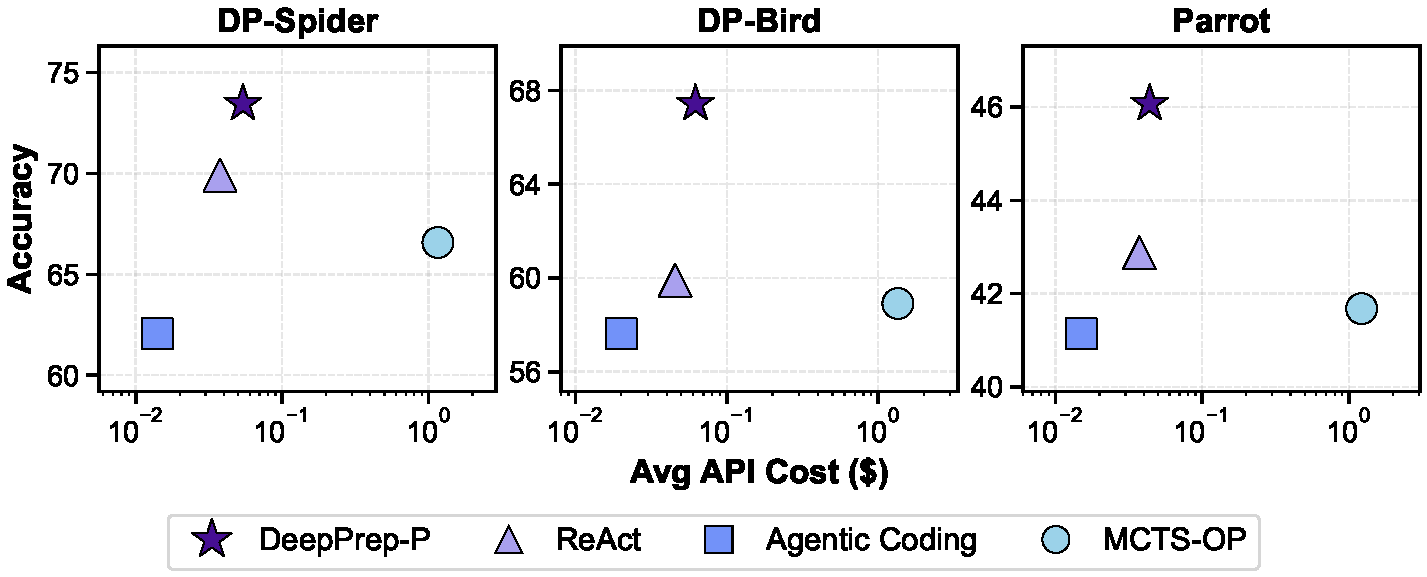
\includegraphics[width=0.99\columnwidth]{plots/plot/acc_cost_tradeoff_claude.pdf}
    \vspace{-1em} 
    \caption{Comparison of \sys and baselines based on Claude-4 on Accuracy and API cost.}
    \label{fig:acc_cost_tradeoff_claude}
  \vspace{-0.5em}
\end{figure}
\begin{figure}[t]
    \centering
    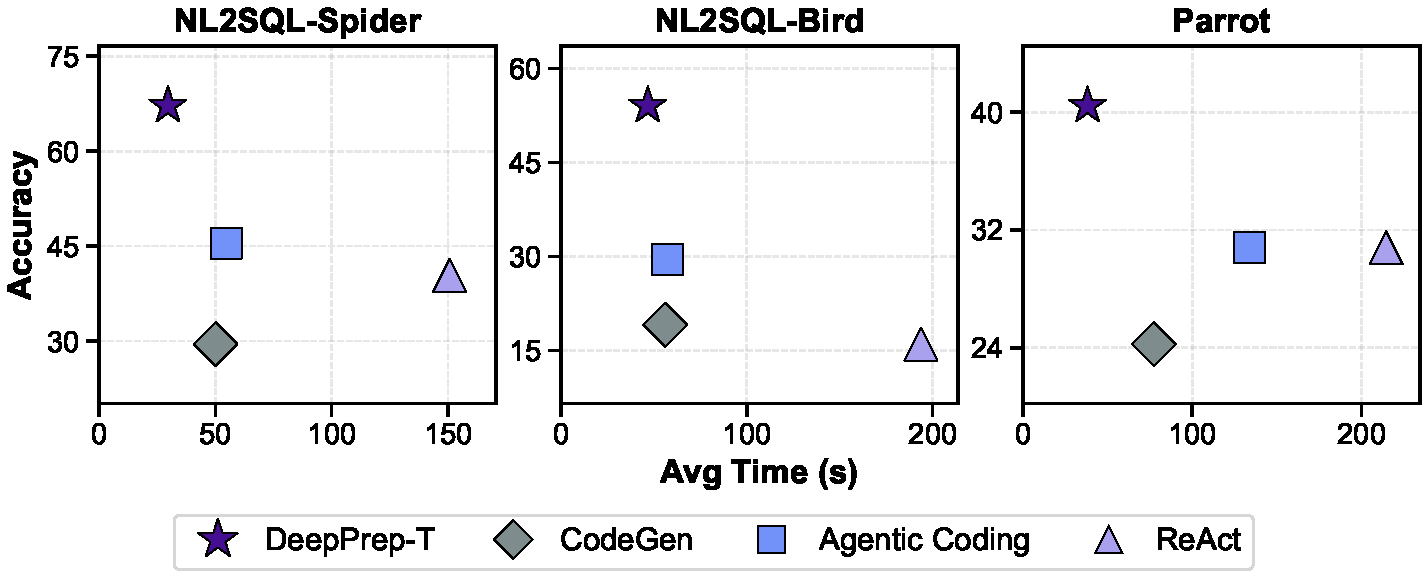
\includegraphics[width=0.99\columnwidth]{plots/plot/time_acc_tradeoff_Qwen3_14B.pdf}
    \vspace{-1em} 
    \caption{Comparison of \syst and baselines based on Qwen3-14B on Accuracy and Time.}
    \label{fig:time_acc_tradeoff_Qwen3_14B}
  \vspace{-0.5em}
\end{figure}

For \sys, we focus on API Cost. Since these methods rely on commercial APIs, latency metrics are often unreliable due to network instability and the opacity of server-side hardware allocation.
For \sys, which are designed for local deployment, users prioritize Inference Latency.

\noindent \textbf{Exp-\expnum\label{exp:acc_cost_tradeoff}: Analysis of the Accuracy \& API Cost Trade-off.}
Figure~\ref{fig:acc_cost_tradeoff_claude} illustrates the trade-off between accuracy and average API cost per case for \sys and the three top-performing baselines in terms of accuracy using Claude-4.
We observe that search-based methods like MCTS-OP incur prohibitive costs. For instance, on the complex DP-Bird dataset, MCTS-OP consumes an average of \textbf{\$1.35} per case while achieving an accuracy of 58.91\%.
In contrast, \sys achieves a significantly higher accuracy of \textbf{67.43\%} with a cost of only \textbf{\$0.062}.
This represents a cost reduction of over \textbf{21$\times$} compared to MCTS-OP.
% Furthermore, compared to linear agents like ReAct, \sys incurs a marginal cost increase (approximately \$0.016 on DP-Bird) yet yields substantial performance gains (+7.52\%).
The superior cost-effectiveness of \sys stems from its agentic reasoning design.
Unlike MCTS-OP relying on statistical rollout simulations to estimate node values, \sys leverages the global state tree to analyze error semantics.
This allows \sys to prune invalid branches rather than relying on blind trial-and-error, thereby optimizing token usage.

\begin{shaded}
\noindent \textbf{Finding \findingnum: \sys achieves the best cost-performance ratio, reducing API costs by $\sim$21$\times$ compared to MCTS-OP while achieving the highest accuracy.}
\end{shaded}

\noindent \textbf{Exp-\expnum\label{exp:acc_time_tradeoff}: Analysis of the Accuracy \& Latency Trade-off.}
% We further evaluate the inference efficiency of the training-based framework \sys by measuring the average time required to complete a task.
% Real-time responsiveness is critical for interactive data preparation sysems.
In Figure~\ref{fig:time_acc_tradeoff_Qwen3_14B}, we compare \sys against the three top-performing prompting baselines under the Qwen3-14B backbone.
We observe that iterative prompting baselines suffer from high latency.
Specifically, ReAct requires an average of {193.62} seconds per case on DP-Bird, resulting in a low accuracy of 16.04\%.
Conversely, \sys completes the same tasks in \textbf{46.76} seconds (\textbf{4$\times$} speedup) while achieving a state-of-the-art accuracy of \textbf{54.09\%}.
This is because ReAct requires more turns to complete complex tasks, since it constraints to output one operator per turn.
Even compared to the non-iterative CodeGen baseline (56.12s), \sys maintains a lower latency while improving accuracy by nearly 35\%.
This efficiency gain is attributed to the operator-assisted design. We only need to generate operators instead of the complete python programs, greatly reducing the overhead if generating new tokens.

\begin{shaded}
\noindent \textbf{Finding \findingnum: \sys demonstrates superior inference efficiency, achieving a 4$\times$ speedup over ReAct on complex datasets.}
\end{shaded}